\documentclass[12pt,halfline,a4paper]{ouparticle}
\usepackage{amsmath,amssymb}
\usepackage[round]{natbib}
\usepackage{graphicx,rotating}
\usepackage{dsfont}
\usepackage{xspace}
\usepackage{booktabs}
\usepackage[binary-units]{siunitx}
\usepackage[section]{placeins}

\newcommand{\Est}[1]{\hat{#1}}

\newcommand{\beginsupplement}{%
        \setcounter{table}{0}
        \renewcommand{\thetable}{S\arabic{table}}%
        \renewcommand{\theHtable}{S\thetable}
        \setcounter{figure}{0}
        \renewcommand{\thefigure}{S\arabic{figure}}%
        \renewcommand{\theHfigure}{S\thefigure}
     }
\newcommand{\stopsupplement}{%
        \setcounter{table}{0}
        \renewcommand{\thetable}{\arabic{table}}%
        \renewcommand{\theHtable}{X\thetable}
        \setcounter{figure}{0}
        \renewcommand{\thefigure}{\arabic{figure}}%
        \renewcommand{\theHfigure}{X\thefigure}
     }

% method names

\newcommand{\Stdpopsim}{\texttt{Stdpopsim}\xspace}
\newcommand{\stdpopsim}{\texttt{stdpopsim}\xspace}
\newcommand{\dadi}{$\partial a \partial i$\xspace}
\newcommand{\MSMC}{\texttt{MSMC}\xspace}
\newcommand{\smcpp}{\texttt{smc++}\xspace}
\newcommand{\stairwayplot}{\texttt{stairway plot}\xspace}
\newcommand{\fastsimcoal}{\texttt{fastsimcoal2}\xspace}
\newcommand{\tskit}{\texttt{tskit}\xspace}

\newcommand{\adk}[1]{\textcolor{red}{ADK: #1}}

\usepackage[hidelinks]{hyperref}
\usepackage[blocks]{authblk}
\renewcommand\Affilfont{\small}
\makeatletter
\renewcommand\AB@affilsepx{, \protect\Affilfont}
\makeatother
\usepackage[utf8]{inputenc}

\usepackage{fancyhdr}
\pagestyle{fancy}
\fancyhf{}
\rhead{\texttt{stdpopsim}}
\lhead{PopSim Consortium}
\fancyfoot[C]{\thepage}

\usepackage{etoolbox}
\pretocmd{\abstractname}{\newpage}{}{}

\usepackage{lineno}
\linenumbers

\begin{document}

\title{A community-maintained standard library of population genetic models}
% First authors
\author[1,$\star$]{Jeffrey R. Adrion}
\author[2,$\star$]{Christopher B. Cole}
\author[3,$\star$]{Noah Dukler}
\author[1,$\star$]{Jared G. Galloway}
\author[4,$\star$]{Ariella L. Gladstein}
\author[5,$\star$]{Graham Gower}
\author[6,$\star$]{Christopher C. Kyriazis}
\author[7,$\star$]{Aaron P. Ragsdale}
\author[8,$\star$]{Georgia Tsambos}
% Second Authors
\author[9]{Franz Baumdicker}
\author[10]{Jedidiah Carlson}
\author[11]{Reed A. Cartwright}
\author[12]{Arun Durvasula}
\author[13]{Ilan Gronau}
\author[14]{Bernard Y. Kim}
\author[15]{Patrick McKenzie}
\author[16]{Philipp W. Messer}
\author[17]{Ekaterina Noskova}
\author[18]{Diego Ortega-Del Vecchyo}
\author[5]{Fernando Racimo}
\author[19]{Travis J. Struck}
%Senior Authors
\author[7,$\dagger$]{Simon Gravel}
\author[19,$\dagger$]{Ryan N. Gutenkunst}
\author[6,$\dagger$]{Kirk E. Lohmueller}
\author[1,$\dagger$]{Peter L. Ralph}
\author[4,$\dagger$]{Daniel R. Schrider}
\author[3,$\dagger$]{Adam Siepel}
\author[20,$\dagger$,$\aleph$]{Jerome Kelleher}
\author[1,$\dagger$,$\aleph$]{Andrew D. Kern}

\affil[1]{Department of Biology and Institute of Ecology and Evolution, University of Oregon}
\affil[2]{Wellcome Trust Centre for Human Genetics, University of Oxford}
\affil[3]{Simons Center for Quantitative Biology, Cold Spring Harbor Laboratory}
\affil[4]{Department of Genetics, University of North Carolina at Chapel Hill}
\affil[5]{Lundbeck GeoGenetics Centre, Globe Institute, University of Copenhagen}
\affil[6]{Department of Ecology and Evolutionary Biology, University of California, Los Angeles}

\affil[7]{Department of Human Genetics, McGill University}
\affil[8]{Melbourne Integrative Genomics, School of Mathematics and Statistics, University of Melbourne}
\affil[9]{Department of Mathematical Stochastics, University of Freiburg}
\affil[10]{Department of Genome Sciences, University of Washington}
\affil[11]{The Biodesign Institute and The School of Life Sciences, Arizona State University}
\affil[12]{Department of Human Genetics, David Geffen School of Medicine, University of California, Los Angeles}
\affil[13]{The Efi Arazi School of Computer Science, The Herzliya Interdisciplinary Center, Israel}
\affil[14]{Department of Biology, Stanford University}
\affil[15]{Department of Ecology, Evolution, and Environmental Biology, Columbia University}
\affil[16]{Department of Computational Biology, Cornell University}
\affil[17]{Computer Technologies Laboratory, ITMO University}
\affil[18]{International Laboratory for Human Genome Research, National Autonomous University of Mexico}
\affil[19]{Department of Molecular and Cellular Biology, University of Arizona}
\affil[20]{Big Data Institute, Li Ka Shing Centre for Health Information and
Discovery, University of Oxford}
\affil[$\star$]{Denotes shared first authorship, listed alphabetically}
\affil[$\dagger$]{Denotes shared senior authorship, listed alphabetically}
\affil[$\aleph$]{Denotes corresponding authors, listed alphabetically}
% JK: didn't bother with the \texttt stuff for stdpopsim in the abstract as it's nearly
% always dropped in production anyway.

\abstract{The explosion in population genomic data demands ever more complex
modes of analysis, and increasingly these analyses depend on sophisticated simulations.
Recent advances in population genetic simulation have made it possible to
simulate large and complex models, but specifying such models for a particular
simulation engine remains a difficult and error-prone task.
Computational genetics researchers currently re-implement simulation models
independently, leading to duplication of effort and inconsistency.
Population genetics, as a field, also lacks standard benchmarks by which new tools for inference might
be measured. Here we describe a new resource, \stdpopsim, that attempts to rectify this situation.
\Stdpopsim is a community-driven open source project, which provides easy access to a standard
catalog of published simulation models from a wide range of organisms
and supports multiple simulation engine backends.
% PopSim assures correctness in our implementations through a mature, community-based quality control pipeline.
We share some examples demonstrating how \stdpopsim
can be used to systematically compare demographic inference methods,
and we encourage an even broader
community of developers to contribute to this growing resource.
}
\date{}

\keywords{Population genetics, Simulation, Inference, Reproducibility}

\maketitle


\section*{Introduction}
While population genetics has always used statistical methods to make inferences from data,
the degree of sophistication of the questions, models, data, and computational approaches
used have all increased over the past two decades. Currently there exist myriad computational methods
that can infer the histories of populations
\citep{gutenkunst2009inferring,li2011inference,excoffier2013robust,schiffels2014inferring, terhorst2017robust,ragsdale2019models},
the distribution of fitness effects \citep{Boyko:2008cr,kim2017inference,tataru2017inference,Fortier703918,Huang2019,Vecchyo770966},
recombination rates \citep{chan2012genome,lin2013fast,Adrion662247,Barroso2019},
and the extent of positive selection in genome sequence data
\citep{eyre2009estimating, alachiotis2012omegaplus,degiorgio2016sweepfinder2,kern2018diplos,sugden2018localization}.
While these methods have increased our understanding of the
impacts of genetic and evolutionary processes, very little has been done to systematically
benchmark the quality of inferences gleaned from computational population genetics.
As large databases of population genetic variation begin to be used to inform public health procedures,
the accuracy and quality of these inferences is becoming ever more important.

Assessing the accuracy of inference methods for population genetics is
challenging in large part because the ``ground-truth'' in question
generally comes not from direct empirical observations, as the relevant
historical processes can rarely be observed, but instead from simulations.
Population genetic simulations are therefore critically important to the
field, yet there has been no systematic attempt to establish community
standards or best practices for executing them. Instead, the general modus
operandi to date has been for individual groups to validate their own
methods using bespoke simulations.
Often these studies focus more on showcasing a novel method than on
rigorously comparing it with competing methods.
Moreover, this situation results in a great deal of duplicated effort,
and contributes to decreased reproducibility and transparency across the entire field.
It is also a barrier to entry to the field, because new researchers can
struggle with
the many steps involved
in implementing a state-of-the-art population genetics simulation,
including identifying appropriate demographic models from the literature,
translating them into input for a simulator, obtaining appropriate genetic
maps, and choosing appropriate values for key population genetic parameters.

A related issue is that it has been challenging to assess the degree to which modeling assumptions
and choices of data summaries can affect population
genetic inferences. Yet there
are clear examples of different methods yielding fundamentally
different conclusions. For example, Markovian coalescent methods applied to human genomes have
suggested large ancient ($>100,000$ years ago) ancestral population sizes and
bottlenecks that have not been detected by other methods based on allele frequency spectra
\citep[see][]{beichman2017comparison}.
These distinct methods differ in how they model, summarize, and optimize fit to
genetic variation data, suggesting that such design choices can greatly affect the
performance of the inference. Furthermore, some methods are likely to
perform better than others under certain scenarios, but
researchers lack principled guidelines for selecting the best method for addressing
their particular questions. The need for empirical
guidance will only increase as researchers
seek to apply population genetic methods to a growing collection of non-model taxa.

For these reasons, we have generated a standardized, community-driven resource
for simulating published demographic models from a number of popular study systems.
This resource, which we call \stdpopsim, makes running
realistic simulations for population genetic analysis a simple matter of
choosing pre-implemented models from a community-maintained catalog.
The \stdpopsim catalog currently contains three organisms: humans,
\emph{Drosophila~melanogaster}, and \emph{Arabidopsis~thaliana}. For each
organism, the catalog contains information on our current understanding of
 the physical organization (e.g., chromosome structure)
of its genome, one or more inferred genetic maps, default population-level parameters (mutation rate and generation time estimates) 
and one or more published demographic models. These available models
and parameters are meant to represent the current standards in the field, however our 
intention is that this resource will evolve as new results become available. Through
either a command line interface or a simple Python API, users can specify which
organism, genetic map, chromosome, and demographic history they are interested in simulating, and the
simulation output from their chosen model is returned.
In this way, \stdpopsim will lower the barrier to high-quality simulation for exploratory analyses,
enable rigorous evaluation of population genetic software,
and contribute to increased reliability of population genetic inferences.


The \stdpopsim library has been developed by the PopSim Consortium using a
distributed open source model, with strong procedures in place
to continue its growth and maintain its quality.
Importantly, we have rigorous quality control methods to ensure that we have
correctly implemented the models as described in their original publication
and have documented methods for others to contribute new modules.
We invite new collaborators to join our community (https://stdpopsim.readthedocs.io/en/latest/development.html).
Below we describe the resource and give
examples of how it can be used to benchmark demographic inference methods.





\begin{figure}[t]
\begin{center}
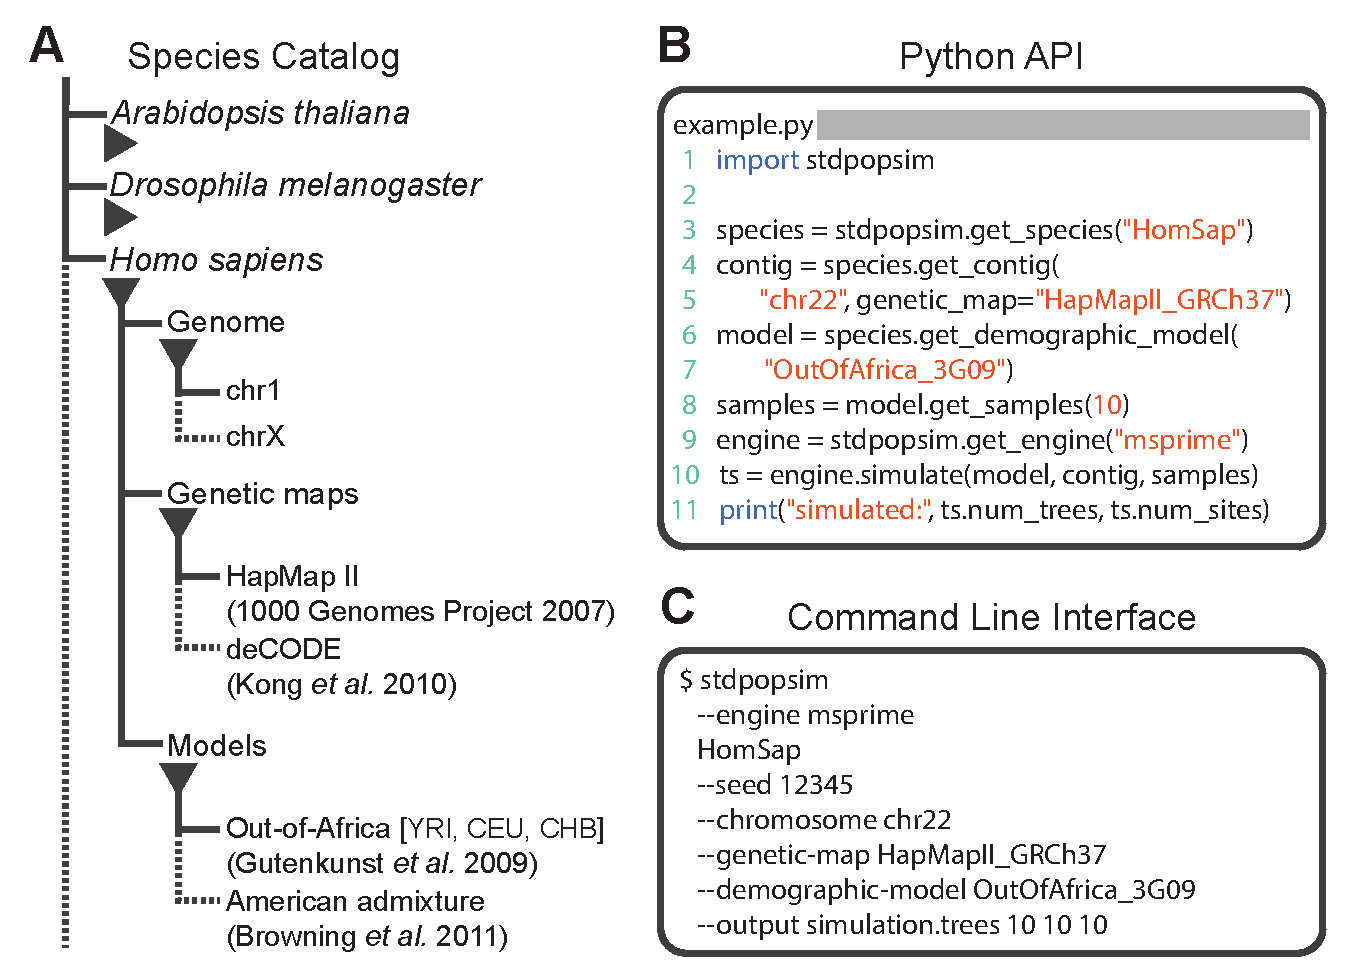
\includegraphics[width=0.7\linewidth]{display_items/Figure1.pdf}
    \caption{\textbf{Structure of \stdpopsim}. \textbf{(A)} The
hierarchical organization of the \stdpopsim catalog contains all model simulation information
within individual species (expanded information shown here for \emph{H.~sapiens} only).
Each species is associated with a representation of the physical genome, and one or more genetic maps and demographic models.
Dotted lines indicate that only a subset of these categories is shown.
At right we show example code to specify
and simulate models using \textbf{(B)} the python API or \textbf{(C)} the command line interface.
    }
\label{fig:cartoon}
\end{center}
\end{figure}

\section*{Results}
\paragraph{The \stdpopsim library.}
The first contribution of the PopSim consortium is \stdpopsim, a
community-maintained library of empirical genome data and population genetics simulation
models. Figure \ref{fig:cartoon} shows a graphical
representation of the structure of \stdpopsim. The package centers
on a catalog of species (Fig.~\ref{fig:cartoon}A), initially consisting of humans,
\textit{D.~melanogaster}, and \textit{A.~thaliana}.
A species definition consists of two key elements.  Firstly, the library defines
some basic information on our current understanding of each 
species' genome, including information about chromosome
lengths, average mutation rate estimates, and generation times. We also provide access to detailed
empirical information such as inferred genetic maps, which model observed
heterogeneity in recombination rate along chromosomes. As such maps are often large,
we do not distribute them directly with the software, but make them available
for download in a standard format. When a simulation using such a map is
requested by the user, \stdpopsim will transparently download the map
data into a local cache,
% (\texttt{$\sim$/.local/cache/stdpopsim} by default on Unix platforms)
where it can be quickly retrieved for subsequent simulations.
In the initial version of \stdpopsim we support
the HapMapII~\citep{international2007second} and
deCODE~\citep{kong2010fine} genetic maps for humans;
the \cite{salome2011recombination} map for \emph{A.~thaliana};
and the \cite{comeron2012many} map for \emph{D.~melanogaster}.
Adding further maps to the library is straightforward.
The second key element of a species description
within \stdpopsim is a set of carefully curated population genetic model
descriptions from the literature, which allow simulation under
specific historical scenarios that have been fit to present-day patterns of
genetic variation (See the Methods for a description of the community
development and quality-control process for these models.)

Given the genome data and simulation model descriptions defined within the
library, it is then straightforward to run standardized simulations
across a range of organisms. \Stdpopsim has a Python API and a user-friendly
command line interface, allowing users with minimal experience direct access to
state-of-the-art simulations. Simulations are output in the ``tree sequence''
format \citep{kelleher2016efficient,kelleher2018efficient,kelleher2019inferring}, which
contains complete genealogical information about the simulated samples, is
extremely compact, and can be processed efficiently using the \tskit library
\citep{kelleher2016efficient,kelleher2018efficient}. The tree sequence format could also be converted
to other formats (e.g., vcf) by the user if desired. Currently,
\stdpopsim uses the  \texttt{msprime} coalescent simulator \citep{kelleher2016efficient}
as the default simulation engine.
We have implemented \texttt{SLiM} \citep{haller2019tree,haller2019slim}
as an alternative backend,
to allow simulation of processes that cannot be modeled under the coalescent.

The \stdpopsim command line interface, by default, outputs citation information
for the models, genetic maps and simulation engines used in any particular run.
We hope that this will encourage users to appropriately acknowledge the
resources used in published work, and encourage authors
publishing demographic models to contribute to our ongoing community-driven development process.
Together with the \stdpopsim version number and the long-term stable identifiers
for population models and genetic maps,
this citation information will result in well-documented and reproducible
simulation workflows. The individual tree sequence files produced by
\stdpopsim also contain complete provenance information including the command
line arguments, operating system environment and versions of key libraries
used.

\subsection*{The Species Catalog}
The central feature of \stdpopsim is the species catalog, a systematic organization
of the key quantitative data needed to simulate a given species. These include a description
of the assembly, information about mutation rate estimates, inferred recombination rate(s), and generation time
in addition to a series of demographic models that have been estimated for that organism.

The current contents of the \stdpopsim catalog are shown in \autoref{tab:catalog}.
These range from
simple, single population histories \cite[e.g.,][]{sheehan2016deep},
to complex models which include population splitting, migration, and archaic
admixture \cite[e.g.,][]{ragsdale2019models}.
In addition to those models shown, at time of writing
the PopSim Consortium has models in development for \textit{Pongo abelii}, \textit{Canis familiaris}, and \textit{Escherichia coli}.

\renewcommand{\arraystretch}{1.2}
\begin{table}[t]
% Make sure the table is centered even though it's too wide
\makebox[\textwidth][c]{
    \begin{footnotesize}
    \begin{tabular}{lllS[table-format=3.1]S[table-format=3.1]S[table-format=2.1]}
\toprule
& Model ID & Citation & 
\multicolumn{1}{c}{ CPU(s) } 
&
\multicolumn{1}{c}{ RAM(MB) } 
&
\multicolumn{1}{c}{ File(MB) } 
\\
\midrule
\multicolumn{6}{l}{ HomSap (\emph{Homo sapiens}) } \\
&
Africa\_1T12& \cite{tennessen2012evolution} & 10.4& 193.3& 23.3\\
&
Zigzag\_1S14& \cite{schiffels2014inferring} & 3.4& 105.0& 7.9\\
&
AshkSub\_7G19& \cite{gladstein2019substructured} & 15.7& 215.3& 26.4\\
&
OutOfAfrica\_3G09& \cite{gutenkunst2009inferring} & 10.9& 181.3& 21.1\\
&
OutOfAfrica\_2T12& \cite{tennessen2012evolution} & 11.3& 198.0& 24.1\\
&
AncientEurasia\_9K19& \cite{kamm2019efficiently} & 69.4& 304.1& 41.2\\
&
AmericanAdmixture\_4B11& \cite{browning2018ancestry} & 11.1& 187.3& 22.3\\
&
PapuansOutOfAfrica\_10J19& \cite{jacobs2019multiple} & 234.7& 526.3& 77.8\\
&
OutOfAfricaArchaicAdmixture\_5R19& \cite{ragsdale2019models} & 9.6& 184.5& 21.7\\
\midrule
\multicolumn{6}{l}{ DroMel (\emph{Drosophila melanogaster}) } \\
&
OutOfAfrica\_2L06& \cite{li2006inferring} & 0.6& 68.7& 1.6\\
&
African3Epoch\_1S16& \cite{sheehan2016deep} & 0.5& 60.9& 0.2\\
\midrule
\multicolumn{6}{l}{ AraTha (\emph{Arabidopsis thaliana}) } \\
&
African2Epoch\_1H18& \cite{huber2018gene} & 434.1& 359.2& 50.7\\
&
African3Epoch\_1H18& \cite{huber2018gene} & 208.6& 400.6& 58.0\\
&
SouthMiddleAtlas\_1D17& \cite{durvasula2017african} & 159.6& 315.4& 43.1\\
\midrule
\multicolumn{6}{l}{ PonAbe (\emph{Pongo abelii}) } \\
&
TwoSpecies\_2L11& \cite{locke2011comparative} & 7.4& 170.5& 14.7\\
\bottomrule
\end{tabular}

    \end{footnotesize}
}
\caption{\label{tab:catalog}
Initial set of demographic models in the Catalog and simple benchmarks.
For each model we report the CPU time, maximum memory usage and the
size of the output \tskit file. In each case we simulate 100 samples
drawn from the first population, for the shortest chromosome of that species
and a constant chromosome-specific recombination rate.
The times reported are for a single run on an Intel i5-7600 CPU.
Computing resources required will vary widely depending on sample sizes, chromosome length,
recombination rates and other factors.
}
\end{table}

Currently, {\em Homo sapiens} has the largest number of population models in
\stdpopsim (see Table \ref{tab:catalog}).
These models include: a simplified version of the \cite{tennessen2012evolution}
model with only the African population specified (expansion from the ancestral
population and recent growth; Africa\_1T12), the three-population model of \cite{gutenkunst2009inferring}
which specifies the out-of-Africa bottleneck as well as the subsequent divergence of
the European and Asian populations (OutOfAfrica\_3G09), the \cite{tennessen2012evolution} two-population variant of the
\citeauthor{gutenkunst2009inferring} model which does not include Asian populations, but more explicitly models
recent rapid human population growth (OutOfAfrica\_2T12), the \cite{browning2018ancestry} admixture model
for American populations which specifies ancestral African, European, and Asian population
components (AmericanAdmixture\_4B11), a three-population out-of-Africa model from \cite{ragsdale2019models}
which includes archaic admixture (OutOfAfricaArchaicAdmixture\_5R19),
a complex model of ancient Eurasian admixture from \cite{kamm2019efficiently} (AncientEurasia\_9K19),
and a synthetic model of oscillating population size from \cite{schiffels2014inferring} (Zigzag\_1S14).
Together these models
contain features believed to have widespread impacts in real data (e.g., bottlenecks, population growth,
admixture) and are therefore highly pertinent in the context of method development.

Beyond humans we have have implemented two demographic models for
\textit{D.~melanogaster}, three from \textit{A.~thaliana}, and are currently developing
models for \textit{P.~abelii} , \textit{Canis familiaris}, and \textit{E.~coli}.
For \textit{D.~melanogaster} we have implemented the three-epoch model estimated by \cite{sheehan2016deep} from
an African sample (African3Epoch\_1S16), as well as the out-of-Africa divergence
and associated bottleneck model of \cite{li2006inferring}, which jointly models African
and European populations (OutOfAfrica\_2L06). For \emph{A. thaliana}, we implemented the
model in \cite{durvasula2017african} inferred using \MSMC. This model includes
a continuous change in population size over time, rather than pre-specified epochs of different
population sizes (SouthMiddleAtlas\_1D17). We have also implemented a two-epoch and a three-epoch model estimated from African
samples of \emph{A. thaliana} in \cite{huber2018gene} (African2Epoch\_1H18 and African3Epoch\_1H18).
%For \emph{P. pygmaeus} we have implemented the two
%species divergence model of \cite{locke2011comparative}, which models isolation with migration between \emph{P. pygmaeus}
%and \emph{P. abelii}.
%For \emph{E. coli} we have a simple, large constant population size model implemented.
In addition to organism-specific models, \stdpopsim also includes a generic piecewise constant size model and
isolation with migration (IM) model which can be used with any genome and genetic map.

To guarantee reproducibility,
we have standardized naming
conventions for species, genetic maps, and demographic models that will enable long-term stability
of unique identifiers used throughout \stdpopsim,
as described in our documentation
(\url{https://stdpopsim.readthedocs.io/en/latest/development.html#naming-conventions}).


\subsection*{Use case: comparing methods of demographic inference}

As an example of the utility of \stdpopsim, we demonstrate how it can be used
to easily and fairly compare popular demographic inference methods.
Although we present comparison of results from several
methods, our aim at this stage is not to provide an exhaustive
evaluation or ranking of these methods. Our hope is instead that future work built upon this resource
will enable more detailed exploration of the strengths and weaknesses of the numerous
inference methods that are available to the population genetics community
(see Discussion).

We start by comparing popular methods for estimating
population size histories ($N(t)$) of single populations and subsequently
show simple examples of multi-population inference.
To reproducibly evaluate and compare the performance of inference methods, we developed
workflows using \texttt{snakemake} \citep{koster2012snakemake}
that are available from \url{https://github.com/popsim-consortium/analysis},
that allow efficient computing in multicore or cluster environments.

For single-population population size histories, we compared
\MSMC~\citep{schiffels2014inferring}, \smcpp~\citep{terhorst2017robust}, and
\stairwayplot~\citep{liu2015exploring}
 on simulated genomes sampled from a single population,
in a number of the demographic models described above.
Our workflow generates $R$ replicates of $C$ chromosomes, producing $n$ samples in each of a total of $R \times C$
simulations for each demographic model. After simulation, the workflow prepares
input files for each inference method by grouping all
chromosomes, for each sample, into a single file. For each of the $R$ simulation replicates, this step results in an
input file for each of the
respective inference methods and derived from the same simulated tree sequences.
Each of the inference programs are then run in parallel, followed by plotting of
$N(t)$ estimates from each program.

\begin{figure}
\begin{center}
\includegraphics[width=0.8\linewidth]{display_items/homo_sapiens_mask_Ragsdale.png}
\caption{\textbf{Comparing estimates of $N(t)$ in humans}. Here we show estimates of population
size over time ($N(t)$) inferred using 4 different methods: \smcpp, \texttt{stairway plot}, and
\MSMC with $n=2$ and $n=8$. Data were generated by simulating
replicate human genomes under the OutOfAfricaArchaicAdmixture\_5R19 model and using the
HapMapII\_GRCh37 genetic map~\citep{international2007second}. From top to bottom we show estimates for each
of the three populations in the model (YRI, CEU, and CHB). In shades of blue we show the estimated
$N(t)$ trajectories for each replicate.
As a proxy for the truth, in black we show inverse coalescence rates
as calculated from the true demographic model (see text).
}
\label{fig:n_t_ragsdale}
\end{center}
\end{figure}


Figure \ref{fig:n_t_ragsdale} presents the results
from simulations under OutOfAfricaArchaicAdmixture\_5R19,
a model of human migration out of Africa that includes archaic admixture
\citep{ragsdale2019models}, along with an empirical genetic map. In each column of this figure
we show $N(t)$ inferred from samples taken from each of the three extant populations in the model.
In each row we show comparisons among the methods (including two sample sizes for \MSMC).
Blue lines show estimates from each of three replicate whole genome simulations and (FIXME: what color?)
lines show the simulated population sizes. When fitting single-population models to data simulated for multiple
populations with migration, however, we do not necessarily expect the inference methods to recover the 
``true'' simulated population size due to model misspecification. Instead, many methods work by matching
 coalescence time distributions, and a single-population model with varying population size can match any 
 coalescence time distribution (in which case coalescence rate is the inverse of the effective size).
For this reason, we also plot the inverse coalescence rates calculated analytically in \texttt{msprime} (see Appendix)
as another benchmark of the ``truth'' in the single-population inference setting. 
While there is variation in accuracy among methods, populations, and individual replicates,
the methods are generally accurate for this model of human history.

Using \stdpopsim, we can readily compare performance on this benchmark to
that based on a different model of human history. In Figure \ref{fig:n_t_gutenkunst} we show estimates of
$N(t)$ from simulations using the same physical and genetic maps, but from the OutOfAfrica\_3G09
demographic model that does not include archaic admixture. Again we see that each
of the methods is capturing relevant parts of the population history, although the
accuracy varies across time. In comparing inferences between the
models it is interesting to note that $N(t)$ estimates for the CHB and CEU
simulated populations are generally better across methods than estimates from the YRI
simulated population.

We can also
see how well methods might do at recovering the population history of a constant-sized population,
with human genome architecture and genetic map.
We show results of such an
experiment in Figure \ref{fig:n_t_HomSap_constant}.
All methods recover population size within a factor of two of the truth, however
SMC-based methods, perhaps due to their regularization, tend to infer sinusoidal
patterns of population size even though no such change is present.


\begin{figure}
\begin{center}
\includegraphics[width=0.8\linewidth]{display_items/d_mel_Sheehan_mask2.png}
\caption{\textbf{Comparing estimates of $N(t)$ in \textit{Drosophila}}. Population
size over time ($N(t)$) estimated from an African population sample. Data were generated by simulating
replicate \textit{D.~melanogaster} genomes under the African3Epoch\_1S16 model
with the genetic map of \cite{comeron2012many}. In shades of blue we show the estimated
$N(t)$ trajectories for each replicate.
As a proxy for the truth, in black we show inverse coalescence rates
as calculated from the true demographic model (see text).
}
\label{fig:n_t_sheehan}
\end{center}
\end{figure}

As most method development for population genetics has been focused on human
data, it is of consequence to ask how such methods might perform in non-human
genomes. Figure \ref{fig:n_t_sheehan} shows parameter estimates from the African3Epoch\_1S16
model, originally estimated from an African sample of \textit{D.~melanogaster} \citep{sheehan2016deep},
and Figure \ref{fig:n_t_AraTha} shows estimates from simulations of \textit{A.~thaliana}
under the African2Epoch\_1H18 model originally inferred by \cite{huber2018gene}.
In both cases, as with humans, we use \stdpopsim to simulate replicate genomes using an empirically-derived genetic map,
and try to infer back parameters of the simulation model.
Accuracy is mixed among methods when doing inference on simulated data from these \textit{D.~melanogaster}
and \textit{A.~thaliana} models, and generally worse than what we
observe for simulations of the human genome.


\begin{figure}
\begin{center}
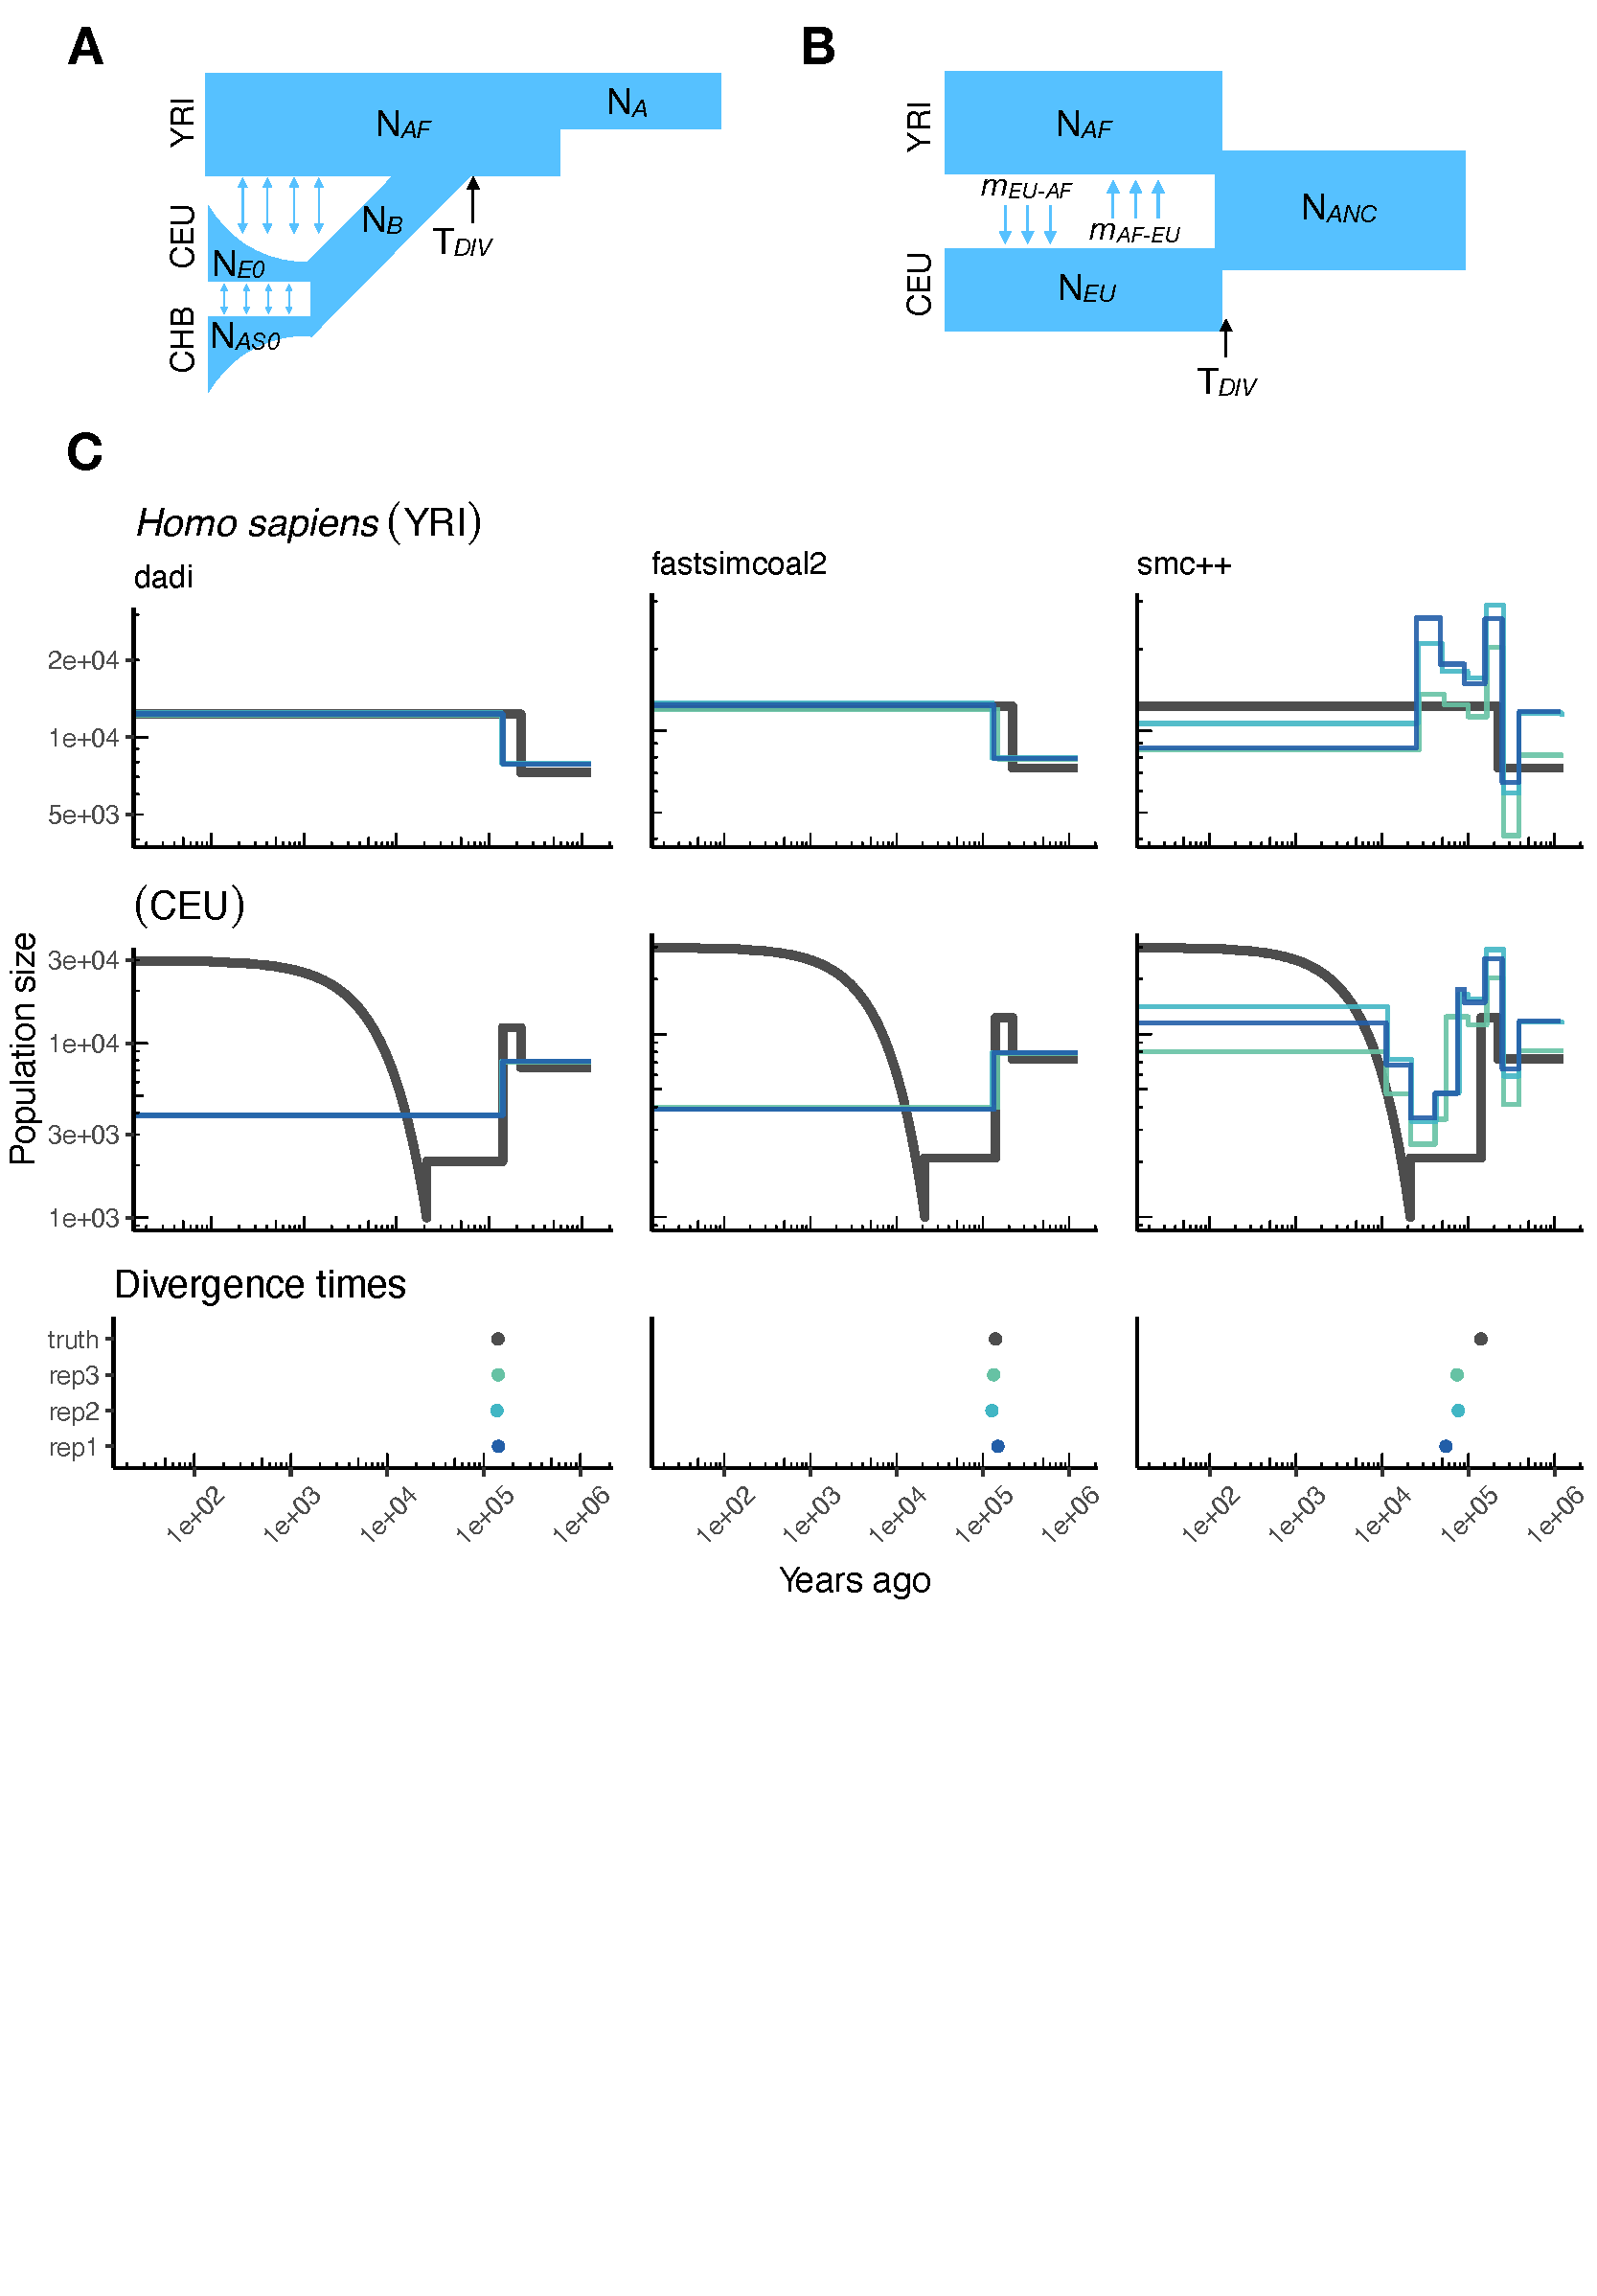
\includegraphics[width=0.7\linewidth]{display_items/homo_sapiens_two_pop_comp.pdf}
\caption{\textbf{Parameters estimated using a multi-population human model}.
Here we show estimates of $N(t)$ inferred using \dadi, \fastsimcoal, and \smcpp. \textbf{(A)} Data were generated by simulating
replicate human genomes under the OutOfAfrica\_3G09 model and using the HapMapII\_GRCh37 genetic map
inferred in \cite{international2007second}. \textbf{(B)} For \dadi and \fastsimcoal we show parameters inferred
by fitting the depicted IM model, which includes population sizes, migration rates, and a split
time between CEU and YRI samples. \textbf{(C)} Population size estimates for each population (rows)
from \dadi, \fastsimcoal, and \smcpp (columns).
In shades of blue we show $N(t)$ trajectories estimated from each simulation,
and in black simulated population sizes for the respective population.
The population split date, $T_{DIV}$, is shown at
the bottom, with a common $x$-axis to the population size panels.}
\label{fig:IM_popn_human}
\end{center}
\end{figure}

\paragraph*{Multi-population demographic models.}
As \stdpopsim implements multi-population demographic models, we also
explored parameter estimation of population divergence parameters. In particular,
we simulated data under multi-population models for humans and \textit{D.~melanogaster}
and then inferred  parameters using \dadi, \fastsimcoal, and \smcpp.
For simplicity, we conducted inference in \dadi and \fastsimcoal by fitting an isolation with migration (IM) model
with constant population sizes and bi-directional migration \citep{hey2004im}. Our motivation for using
an IM model was to mimic the approach often used on empirical datasets, where a relatively
simple model is fit that may not reflect the true underlying demography.
For human models with more than two populations (e.g., \cite{gutenkunst2009inferring})
this means that we are inferring parameters for a model that does
not match the model from which the data were generated (Figures
\ref{fig:IM_popn_human}A and B). However, because model misspecification 
here is less severe  compared to the single-population case, we compare
our inferred population sizes only to the simulated population sizes (black line in
Figure \ref{fig:IM_popn_human}C) and not the inverse coalescence rates.

In Figure \ref{fig:IM_popn_human}C we show estimates of population sizes and divergence
time, for each of the inference methods, using samples drawn from African and European populations
simulated under the OutOfAfrica\_3G09 model. Our results highlight many
of the strengths and weaknesses of the different types of methods we used.
For instance, the SFS-based approaches where we fit simple IM models do not capture
recent exponential growth in the CEU population, but do consistently recover the
simulated YRI population size history. Moreover, these approaches allow for estimating
migration rates (Figure \ref{fig:homsap_mig_rates}), also leading to more accurate inference
of divergence times. However, these migration rate estimates are somewhat biased likely
due to model misspecification (Figure \ref{fig:homsap_mig_rates}).
In contrast, \smcpp is much better at capturing the recent exponential
growth in the CEU population, though the inferred population sizes are generally
noisier. In addition, the assumption of no migration by \smcpp leads to divergence time
estimates that are consistently underestimated (Figure \ref{fig:IM_popn_human}C).

Again, we can compare between species and look at the performance of these methods
for a two-population model of \textit{D.~melanogaster}. Figure
\ref{fig:two_popn_fly} shows inference results using data simulated under 
the OutOfAfrica\_2L06 model. This model includes an ancestral population in
Africa from which a European population splits off following a bottleneck, with no 
post-divergence gene flow between the African and European population (Figure \ref{fig:two_popn_fly}A).
Here again, we find that \dadi and \fastsimcoal infer more consistent histories,
but ignore the brief population bottleneck in Europe. In addition, \dadi
and \fastsimcoal both do reasonably well at correctly inferring the absence of
migration (Figure \ref{fig:dromel_mig_rates}). In contrast, the inferred
demographic parameters from \smcpp are more noisy, though in some cases better
capture the short bottleneck in the European population.

Although these results do not represent an exhaustive benchmarking,
we have highlighted some of the strengths and weaknesses of these methods.
Future work should build on these results and undertake more in-depth comparisons
under a wider range of simulated demographic models.

%%%%%%%%%%%%%%%%%%%%%%%%%%%%%%%%%%%%
\section*{Discussion}

Here we have described the first major product from the PopSim Consortium:
the \stdpopsim library. We have founded the Consortium with a number of specific goals in mind:
standardization of simulation within the population genetics community,
increased reproducibility and ease of use of complex simulations,
community-based development and decision making guiding best practices in population genetics,
and benchmarking of inference methods.

The \stdpopsim library allows for rigorous
standardization of complex population genetic simulations. Population genetics, as a field,
has yet to coalesce around a set of standards for the crucial task of method
evaluation, which in our discipline hinges on simulation. In contrast, other fields such as
structural biology \citep{moult1995large} and machine learning \citep{russakovsky2015imagenet} have a long track record
of standardized method testing. We hope that our efforts represent the beginning of what
will prove to be an equally longstanding and valuable tradition in population genetics.

%Individual research groups are often in the position of having to independently
%reimplement complex, previously published demographic models.
%Additional layers of realism (e.g., recombination maps) make this especially daunting.
%\stdpopsim aims to lower this barrier
%by creating a quality controlled, easy-to-use, gateway to models and organisms
%that are central to modern research in genetics.

We have illustrated in this paper how \stdpopsim can be used for direct
comparisons of inferential methods on a common set of simulations. Our
benchmarking comparisons have been limited, but nevertheless
reveal some informative features. For
example, at the task of estimating $N(t)$ trajectories for simulated human
populations, we find that the sequence-based methods (\MSMC and \smcpp)
perform somewhat better overall---at least for mid-range values of
$t$---than the site frequency spectrum-based method (\stairwayplot)
(Figures~\ref{fig:n_t_ragsdale} and~\ref{fig:n_t_gutenkunst}), which
tends to over-estimate the sizes of oscillations.  In contrast,
\stairwayplot outperforms the sequence-based methods
on simulations of \textit{D.~melanogaster} or \textit{A.~thaliana} populations,
in which linkage disequilibrium is reduced (Figures~\ref{fig:n_t_sheehan} \& \ref{fig:n_t_AraTha}).
In simulations of two human populations
(Figure~\ref{fig:IM_popn_human}), most methods do reasonably well at
reconstructing the simulated YRI history, but struggle with the more complex simulated CEU
history, in large part because of the restriction of constant population sizes.
An exception is \smcpp, which does not have the same
restrictions on its inferred history, and as a result does somewhat better
with the CEU history but tends to overfit the YRI history.
The results for
the two-population \textit{D.~melanogaster} model (Figure~\ref{fig:two_popn_fly})
are generally similar.
In these comparisons, \fastsimcoal and \dadi perform almost identically, which is expected because they fit the same models to the same summaries of the data, differing only in how they calculate model expectations and optimize parameters.

All methods for inferring demographic history have strengths and weaknesses (as recently reviewed by \citet{beichman2018review}.)
We compared inferences from simulated whole genome data, but many factors affect choice of methodology.
Markovian coalescent methods (\MSMC and \smcpp) require long contiguous stretches of sequence data.
In contrast, frequency spectrum methods (\stairwayplot, \dadi, and \fastsimcoal) can use reduced-representation sequencing data, such as RADseq \citep{andrews2016radseq}.
\dadi and \fastsimcoal require a pre-specified parametric model, unlike \MSMC, \smcpp, and \stairwayplot.
Using a parametric approach yields less noisy results, but a model that is too simple may not capture important demographic events (Figures~\ref{fig:IM_popn_human} and~\ref{fig:two_popn_fly}).
From a software engineering perspective, methods also differ in their ease of installation and use.
We hope our workflows will assist in the application of all the methods we have considered.

Altogether, these preliminary experiments highlight
the utility of \stdpopsim for comparing a variety of inference methods on
the same footing, under a variety of different demographic models.
In addition, the ability of \stdpopsim to generate data with and without significant features, such
as a genetic map or population size change (e.g., Figure \ref{fig:n_t_HomSap_constant}), allows
investigation of the failure modes of popular methods.
Moreover the comparison of methods across the various genome organizations, genetic maps,
and demographic histories of different organisms, provides valuable information
about how methods might perform on non-human systems.
Finally, comparison of results across methods or simulation runs
provides an estimate of inference uncertainty, analogous to parametric
bootstrapping,
especially since different methods are likely vulnerable to model misspecification
in different ways.

\Stdpopsim is intended to be a fully open, community-developed project.
Our implementations of genome representations and genetic maps for the some of
the most common study systems in computational genetics---humans, \textit{Drosophila},
and \textit{Arabidopsis} (among others)---are only intended to be a starting point for
future development.  In addition to other taxa,
we plan to incorporate other common biological processes
such as selection, gene conversion, and mutational heterogeneity.
Researchers are invited to contribute to the resource by adding their
organisms and models of choice. The \stdpopsim resource is
accompanied by clearly documented standard operating procedures that are
intended to minimize barriers to entry for new developers.  In this way, we
expect the resource to expand and adapt to meet the evolving needs of the
population genomics community.


% \paragraph{The problem of comparison} % Moved from the intro
% Benchmarking the performance of inference methods in population genetics is not straightforward.
% Different methods often fit different types of model
% or use different summaries of the genetic variation data, even when
% attempting to address the same biological question. For example, there are
% numerous methods to infer population size changes.
% The \MSMC method \citep{schiffels2014inferring} allows for the
% population to continuously change in size over time. Other methods, such as
% \dadi \citep{gutenkunst2009inferring}, allow for a smaller number of size changes to occur at certain
% points throughout the population's history. The types of data that the
% methods use also differs. While \MSMC uses one to four whole genome sequences and leverages the
% spatial patterns of genetic variation along the sequence, \dadi  instead uses the
% site frequency spectrum (SFS), which summarizes the frequencies of SNPs in the
% sample, ignoring any information about the correlation structure (linkage
% disequilibrium) among SNPs. Thus from the start these methods may not be
% expected to perform equally well in all scenarios,
% and indeed, it is not always clear how to compare to the truth --
% for instance, how well can a method of piecewise constant population sizes
% describe a period of exponential growth?
% Or, how should discrete population models be mapped onto real-world (continuous) geography?
% The answer depends on determining what is most important for the question at hand.

\section*{Methods}
%\subsection*{Generating the PopSim resource}
% RNG: No need to empty subsection.

\subsection*{Model quality control}
As a consortium we have agreed to a standardized procedure for model inclusion
into \stdpopsim that allows for rigorous quality control. Imagine Developer A
wants to introduce a new model into \stdpopsim. Developer A implements the
demographic model for the relevant organism along with clear documentation
of the model parameters and populations. This model is submitted as a ``pull request'',
where it is evaluated by a reviewer and then included as `preliminary',
but is not linked to the online documentation nor the command line interface.
Developer A submits a quality control (QC) issue, after which a second developer,
Developer B, then independently reimplements the model from the relevant
primary sources and adds an automatic unit test for equality between the
QC implementation and the preliminary production model. If the two
implementations are equivalent, the original model is included in \stdpopsim.
If not, we move to an arbitration process whereby A and B first try
to work out the details of what went wrong. If that fails, the original
authors of the published model must be contacted
to resolve ambiguities.
% This process can lead to cycles of revision of the implementation from Developers A and B but allows the project to assure quality.
% Indeed we have already had a number of interesting cases of arbitration to this point.
Further details of our QC process can be found in our developer documentation
(\url{https://stdpopsim.readthedocs.io/en/latest/development.html#}).

\subsection*{Workflow for analysis of simulated data}
To demonstrate the utility of \stdpopsim we created \texttt{Snakemake}
workflows \citep{koster2012snakemake} that perform demographic inference on
tree sequence output from our package using a few common software packages (see Figure \ref{fig:n_t_dag} for an example workflow).
Our choice of \texttt{Snakemake} allows complete reproducibility of the
analyses shown, and all code is available from \url{https://github.com/popsim-consortium/analysis}.

We performed two types of demographic inference.
Our first task was to infer effective population size over time ($N(t)$).
This was done using three software packages: \stairwayplot,
which uses site frequency spectrum information only \citep{liu2015exploring};
\MSMC~\citep{schiffels2014inferring},
which is based on the sequentially Markovian coalescent (SMC),
run with two different sample sizes ($n = 2 , 8$);
and \smcpp~\citep{terhorst2017robust},
which combines information from the site frequency spectrum with
recombination information as in SMC-based methods. No attempt
was made at trying to optimize the analysis from
any particular software package,
as our goal was not to benchmark performance of methods but
instead show how such benchmarking could be easily done using
the \stdpopsim resource. In this spirit we ran each software package as near
to default parameters as possible. For \stairwayplot we
set the parameters ``numRuns=1'' and ``dimFactor=5000''. For \smcpp we used the
``estimate" run mode to infer $N(t)$ with all other parameters set
to their default values. For \MSMC we used the ``--fixedRecombination"
option and used the default number of iterations.

For the single-population task we ran human (HomSap) simulations
using a variety of models (see Table 1): OutOfAfricaArchaicAdmixture\_5R19, OutOfAfrica\_3G09,
a constant-sized generic model, and a two-epoch generic model where the
population size instantaneously decreased from $N=10^4$ to $N=10^3$
five hundred generations before the present. Each HomSap simulation was run
using the HapmapII\_GRCh37 genetic map. For \textit{D.~melanogaster}
we estimated $N(t)$ from an African sample simulated under the DroMel,
African3Epoch\_1S16 model using the Comeron2012\_dm6 map.
Finally, we ran simulations of \emph{A. thaliana} genomes using the
AraTha African2Epoch\_1H18 model under the Salome2012\_TAIR7 map.
For each model, three replicate whole genomes were
simulated and the population size estimated from those data. In all cases we
set the sample size of the focal population to $N=50$ chromosomes.

Following simulation, low-recombination portions of chromosomes were masked
from the analysis in a manner that reflects the ``accessible" subset of sites
used in empirical population genomic studies \citep[e.g.,][]{danecek20111000,langley2012genomic}.
Specifically we masked all regions of \SI{1}{cM} or greater in the lowest 5th percentile of the empirical
distribution of recombination, regions which are nearly uniformly absent for
empirical analysis.

Our second task was to explore inference with two-population models
using some of the multi-population demographic models implemented in \stdpopsim.
For HomSap we used the OutOfAfrica\_3G09 model with the HapmapII\_GRCh37 genetic map,
and for DroMel we used the OutOfAfrica\_2L06 model with the Comeron2012\_dm6 map.
The HomSap model is a three population model (Africa, Europe, and Asia) including post-divergence
migration and exponential growth (Figure \ref{fig:IM_popn_human}C), whereas the
DroMel model is a two population model (Africa and Europe) with no post-divergence
migration and constant population sizes (Figure \ref{fig:two_popn_fly}).

To conduct inference on these models, we applied three commonly used methods:
\dadi~\citep{gutenkunst2009inferring}, \fastsimcoal~\citep{excoffier2013robust},
and \smcpp~\citep{terhorst2017robust}. As above, these methods were used
generally with default settings and we did not attempt to optimize their performance or fit
parameter-rich demographic models.

For both \dadi and \fastsimcoal, we fit a two population
isolation-with-migration (IM) model with constant population sizes.
This IM model contains six parameters:
the ancestral population size, the sizes of each population after the split,
the divergence time, and two migration rate parameters.
Importantly, this meant that for both species, the
fitted model did not match the simulated model (Figures \ref{fig:IM_popn_human} and \ref{fig:two_popn_fly}).
In the HomSap case, we therefore performed inference solely on the Africa
and Europe populations, meaning that the Asia population functioned as a ``ghost''
population that was ignored by our inference. Our motivation for fitting this simple
IM model was to mimic the typical approach of two population inference on empirical
data, where the user is not aware of the `true' underlying demography and the inference
model is often misspecified. To ground-truth our inference approach, we also conducted
inference on a generic IM model that was identical to the model used for inference (Figure \ref{fig:generic_IM}).

From HomSap simulations we took 20 whole genome samples each from the Europe and Africa populations
from each replicate.
Runtimes of DroMel simulations were prohibitively slow when simulating whole genomes
with the Comeron2012\_dm6 map due to large effective population sizes leading to
high effective recombination rates. For this reason, we present only data
from 50 samples of a \SI{3}{\mega\byte} region of chromosome 2R from simulations under OutOfAfrica\_2L06.
For the generic IM simulations, we used the HomSap genome along with the
HapmapII\_GRCh37 genetic map and sampled 20 individuals from each population.

Following simulation, we output tree sequences and masked low-recombination
regions using the same approach described for the single population workflow above. We
converted tree sequences into a two-dimensional site frequency spectrum for all
chromosomes in the appropriate format for \dadi and \fastsimcoal. For each simulation
replicate, we performed 10 runs of \dadi and \fastsimcoal, checking to ensure that 
each method reached convergence. 

Detailed settings for \dadi and \fastsimcoal can be found in the Snakefile
on our git repository (\url{https://github.com/popsim-consortium/analysis}).
Estimates from the highest log-likelihood (out of 10 runs) for each simulation replicate
are shown in Figures \ref{fig:IM_popn_human}C and \ref{fig:two_popn_fly}C.

For \smcpp, we converted the tree sequences into VCF format and performed inference
with default settings. Importantly, \smcpp assumes no migration post-divergence,
deviating from the simulated model.  However, because \smcpp allows
for continuous population size changes, it is better equipped to capture many of the
more complex aspects of the simulated demographic models (e.g., exponential growth).

To visualize our results, we plotted the inferred population size trajectories
for each simulation replicate alongside the simulated population sizes
(Figures \ref{fig:IM_popn_human}C and \ref{fig:two_popn_fly}C).
Here, unlike the single-population workflow,
we compare our inferred population sizes only to the simulated population
sizes and not the inverse coalescence rates. 

\section*{Resource availability}
The version 0.1 release of \stdpopsim is available for download on Github:
\url{https://github.com/popsim-consortium/stdpopsim/releases}.
Documentation for the project can be found here:
\url{https://stdpopsim.readthedocs.io/en/latest/}.




% \subsection*{Extra text}
% [This section describes the stdpopsim Python library. What it’s for, how it’s used and what it can do]
% [First para: running accurate simulations is hard]
% Running realistic population genetic simulations is a complex task today. It is
% straightforward to run simple simulations of population models such as the
% coalescent or Wright-Fisher using (e.g.) msprime or SLiM, but the process of
% instantiating these models to accurately reflect the properties of natural
% populations that are important for a particular study is fraught with
% difficulties. There are typically three important inputs that must be decided:
% the demographic model, recombination and mutation rates. Demographic models for
% a particular species are typically chosen by examining the literature for
% published model specifications, which can consist of dozens of parameters. These
% parameters must be transcribed from the original publication and translated into
% the input format required for the simulator in question. This is a difficult and
% error prone task, and mistakes are common. Recombination and mutation rates are
% simpler to describe and often a single genome-wide estimate is appropriate.
% However, such estimates are updated frequently and there is wide variation in
% the values used for the simulations of the same species. When more fine-grained
% simulations of the local chromosome structure is required, empirical
% recombination and mutation rate maps are used. However, there is no standard
% format for such maps, and finding the maps can be challenging.

\section*{Acknowledgments}
We thank the Probabilistic Modeling in Genomics conference organizers for making this collaboration possible,
and the Simons Center for Quantitative Biology at Cold Spring Harbor Laboratory
for sponsoring the first workshop.
Early on in the project we were encouraged by many people including Patrick Phillips, Richard Durbin,
Dmitri Petrov, and Sohini Ramachandran.
CCK and KEL were funded under NIH Award R35GM119856.
JRA and ADK were funded under NIH Award R01GM117241.
TJS and RNG were funded under NIH Award R01GM127348.
ALG and DRS were funded under NIH award R00HG008696.
ND and AS were supported in part by NIH Awards R01HG010346 and R35GM127070.
FR and GG were supported by a Villum Young Investigator award (project no.~00025300).
DODV is funded by a UC MEXUS-CONACYT Collaborative Grant and a DGAPA-PAPIIT grant (PAPIIT-IA200620).
JK is supported by the Robertson Foundation.


\bibliographystyle{plainnat}
\bibliography{popSim.bib}

\pagebreak
\beginsupplement
\section*{Supplemental Figures}
\begin{figure}
\begin{center}
\includegraphics[width=0.8\linewidth]{display_items/homo_sapiens_mask_Gutenkunst.png}
\caption{\textbf{Comparing estimates of $N(t)$ in humans}. Estimates of population
size over time ($N(t)$) inferred using 4 different methods, \smcpp, \stairwayplot, and
\MSMC with $n=2$ and $n=8$. Data were generated by simulating
replicate human genomes under the \cite{gutenkunst2009inferring} model and using the genetic map
inferred in \cite{international2007second}. From top to bottom we show estimates for each
of the three populations in the model: YRI, CEU, and CHB. In shades of blue we show the estimated
$N(t)$ trajectories for each replicate. In black we show the true population size history as inferred
for the rate of coalescence in the demographic model.}
\label{fig:n_t_gutenkunst}
\end{center}
\end{figure}

\begin{figure}
\begin{center}
\includegraphics[width=0.8\linewidth]{display_items/homo_sapiens_constant.png}
\caption{\textbf{Comparing estimates of $N(t)$ in humans}. Here we show estimates of population
size over time ($N(t)$) inferred using 4 different methods, \smcpp, and \texttt{stairway plot}, and
\MSMC with $n=2$ and $n=8$. Data were generated by simulating
replicate human genomes under a constant sized population model with $N=10^4$ and using the
HapMapII genetic map~\citep{international2007second}. In black we show the true population size history
of the model.}
\label{fig:n_t_HomSap_constant}
\end{center}
\end{figure}

\begin{figure}
\begin{center}
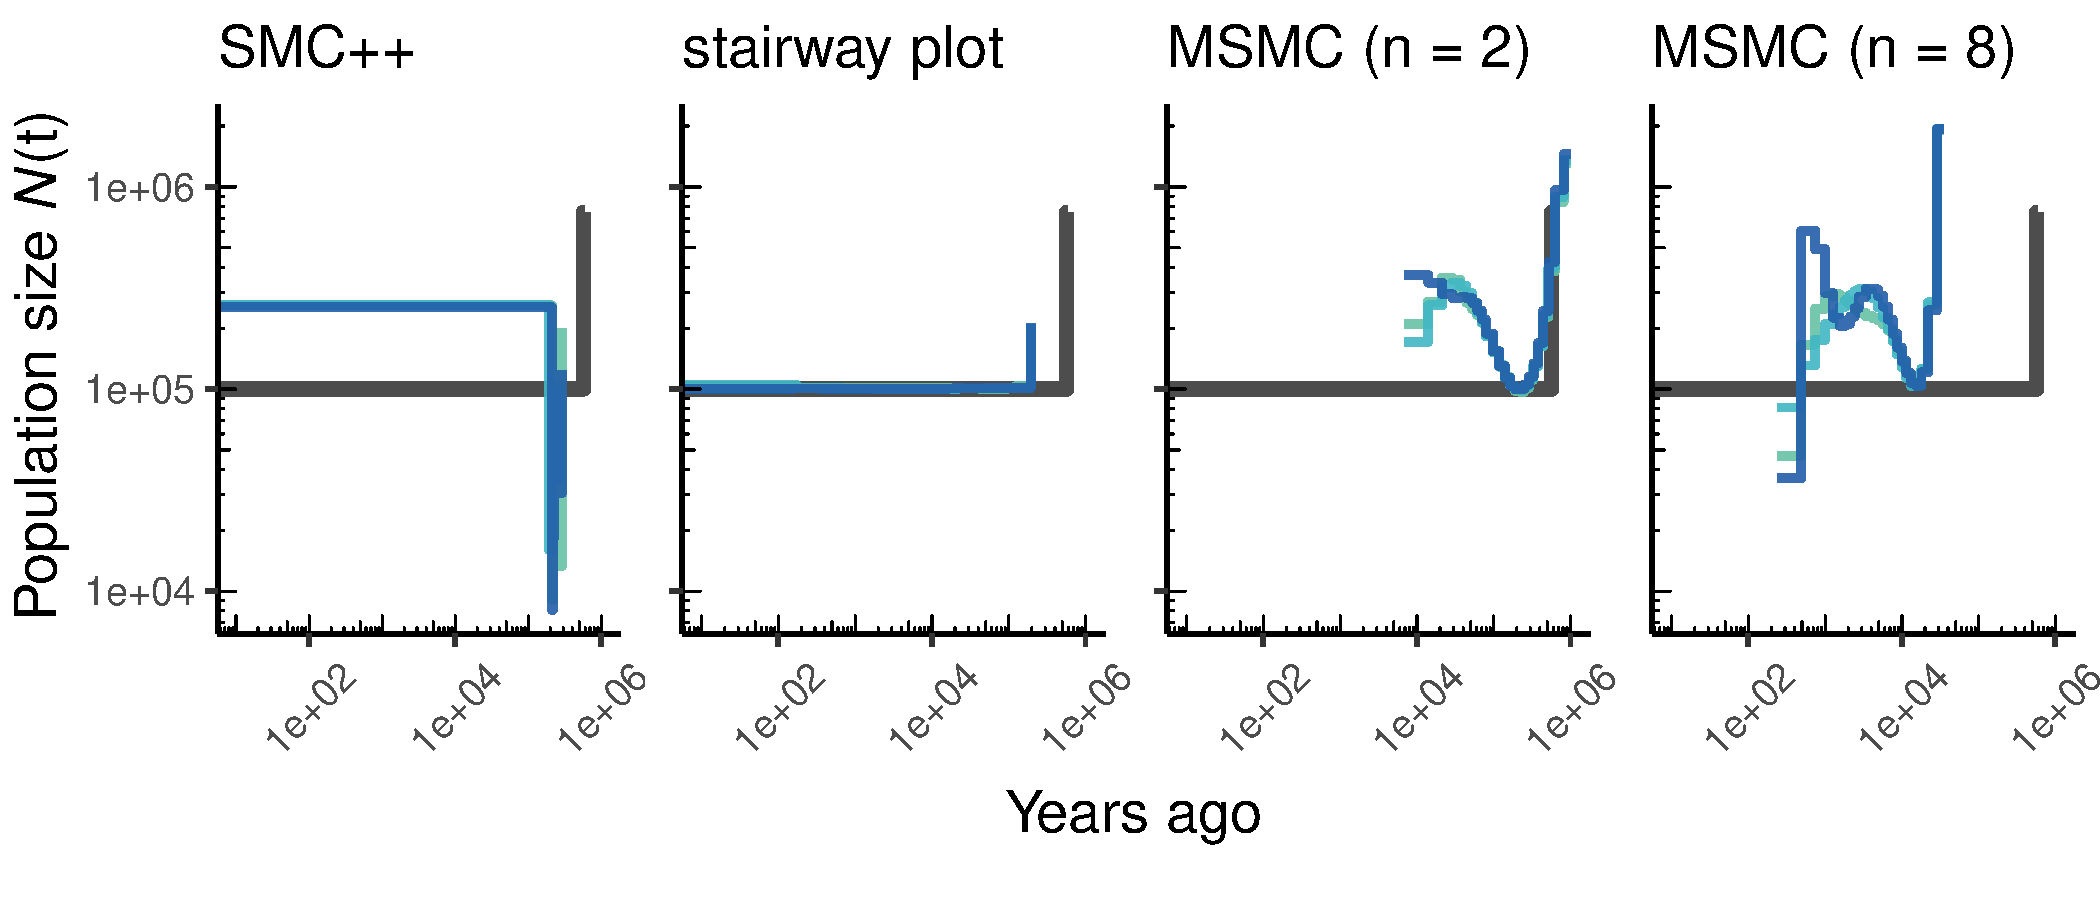
\includegraphics[width=0.8\linewidth]{display_items/AraTha_African2Epoch_1H18.png}
\caption{\textbf{Comparing estimates of $N(t)$ in \textit{A.~thaliana}}. Here we show estimates of population
size over time ($N(t)$) inferred using 4 different methods, \smcpp, and \texttt{stairway plot}, and
\MSMC with $n=2$ and $n=8$. Data were generated by simulating
replicate \textit{A.~thaliana} genomes under the African2Epoch\_1H18 model and using
the genetic map of \cite{salome2011recombination}. In black we show the true population size history
of the model.}
\label{fig:n_t_AraTha}
\end{center}
\end{figure}

\begin{figure}
\begin{center}
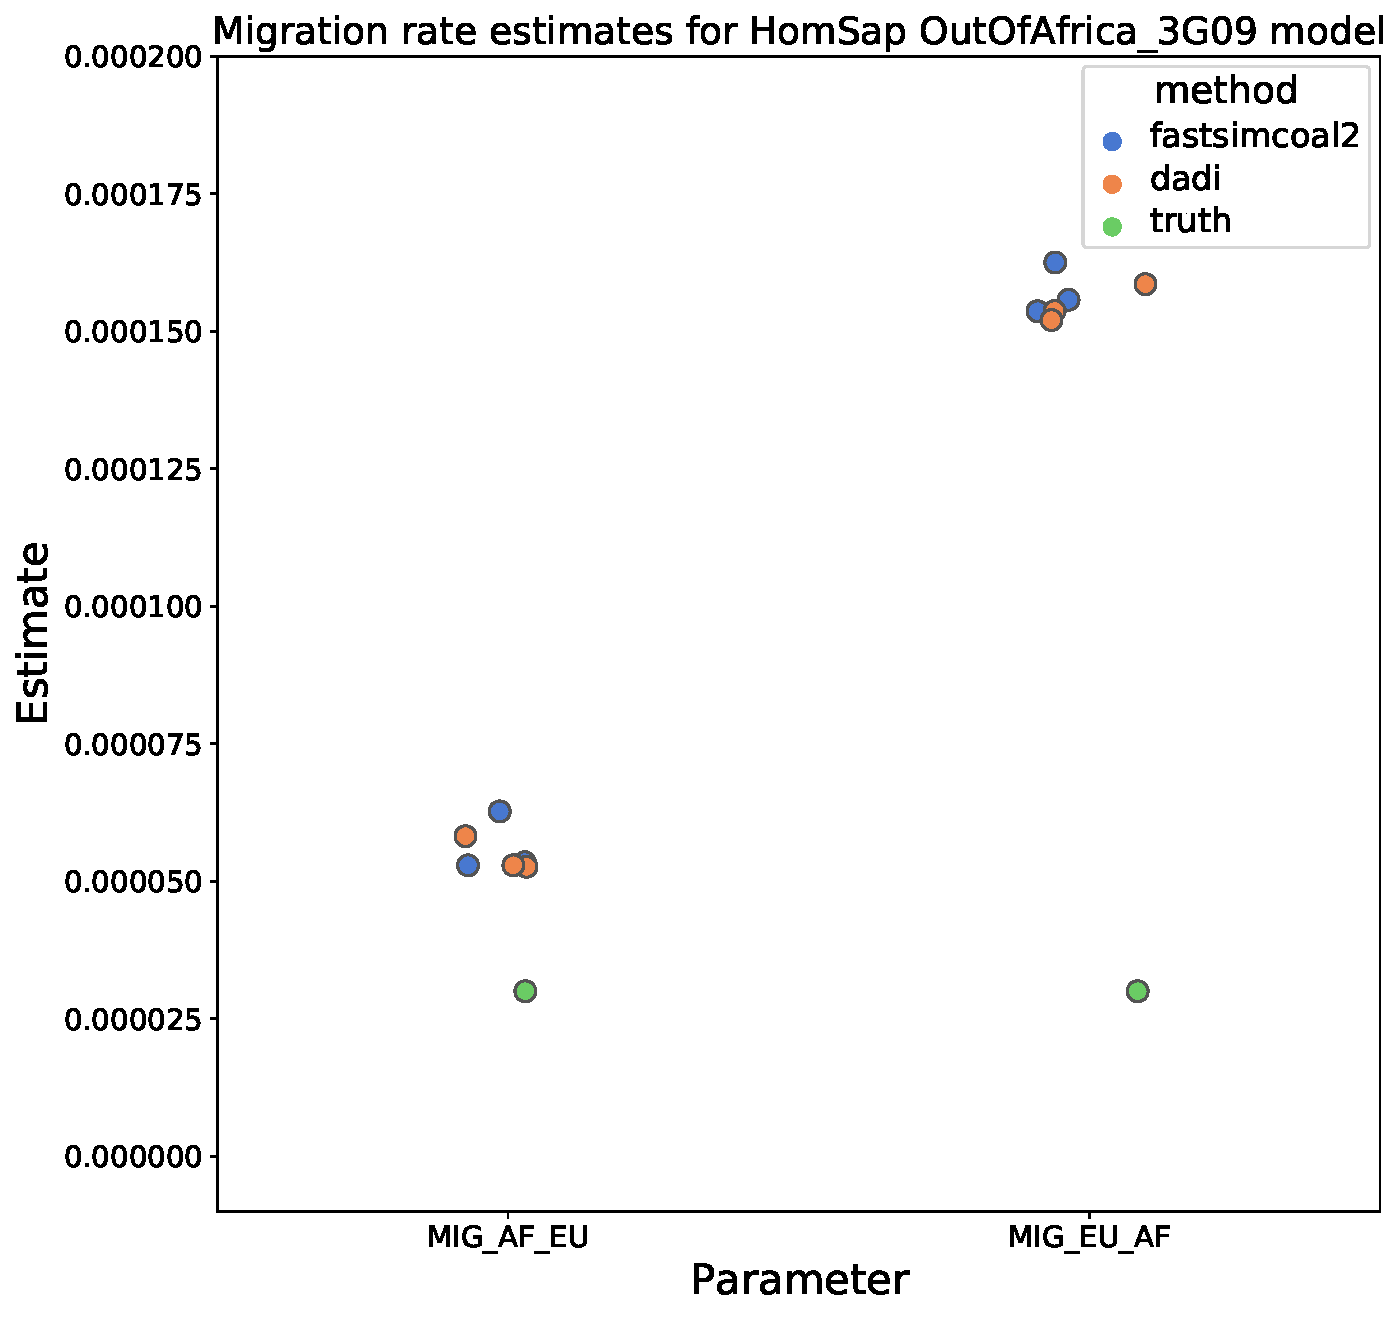
\includegraphics[width=0.8\linewidth]{display_items/homsap_migration_rates.pdf}
\caption{\textbf{Migration rate estimates for the human Gutenkunst model.}
Here we show inferred migration rates from \dadi and \fastsimcoal.
Data were generated by simulating
replicate human genomes under the \cite{gutenkunst2009inferring} model and using the genetic map
inferred in \cite{international2007second}.
Directional migration from Europe to Africa is represented as $MIG\_AF\_EU$ and
migration from Africa to Europe is represented as $MIG\_EU\_AF$.
Note that the $x$-axis coordinates are arbitrary.}
\label{fig:homsap_mig_rates}
\end{center}
\end{figure}


\begin{figure}
\begin{center}
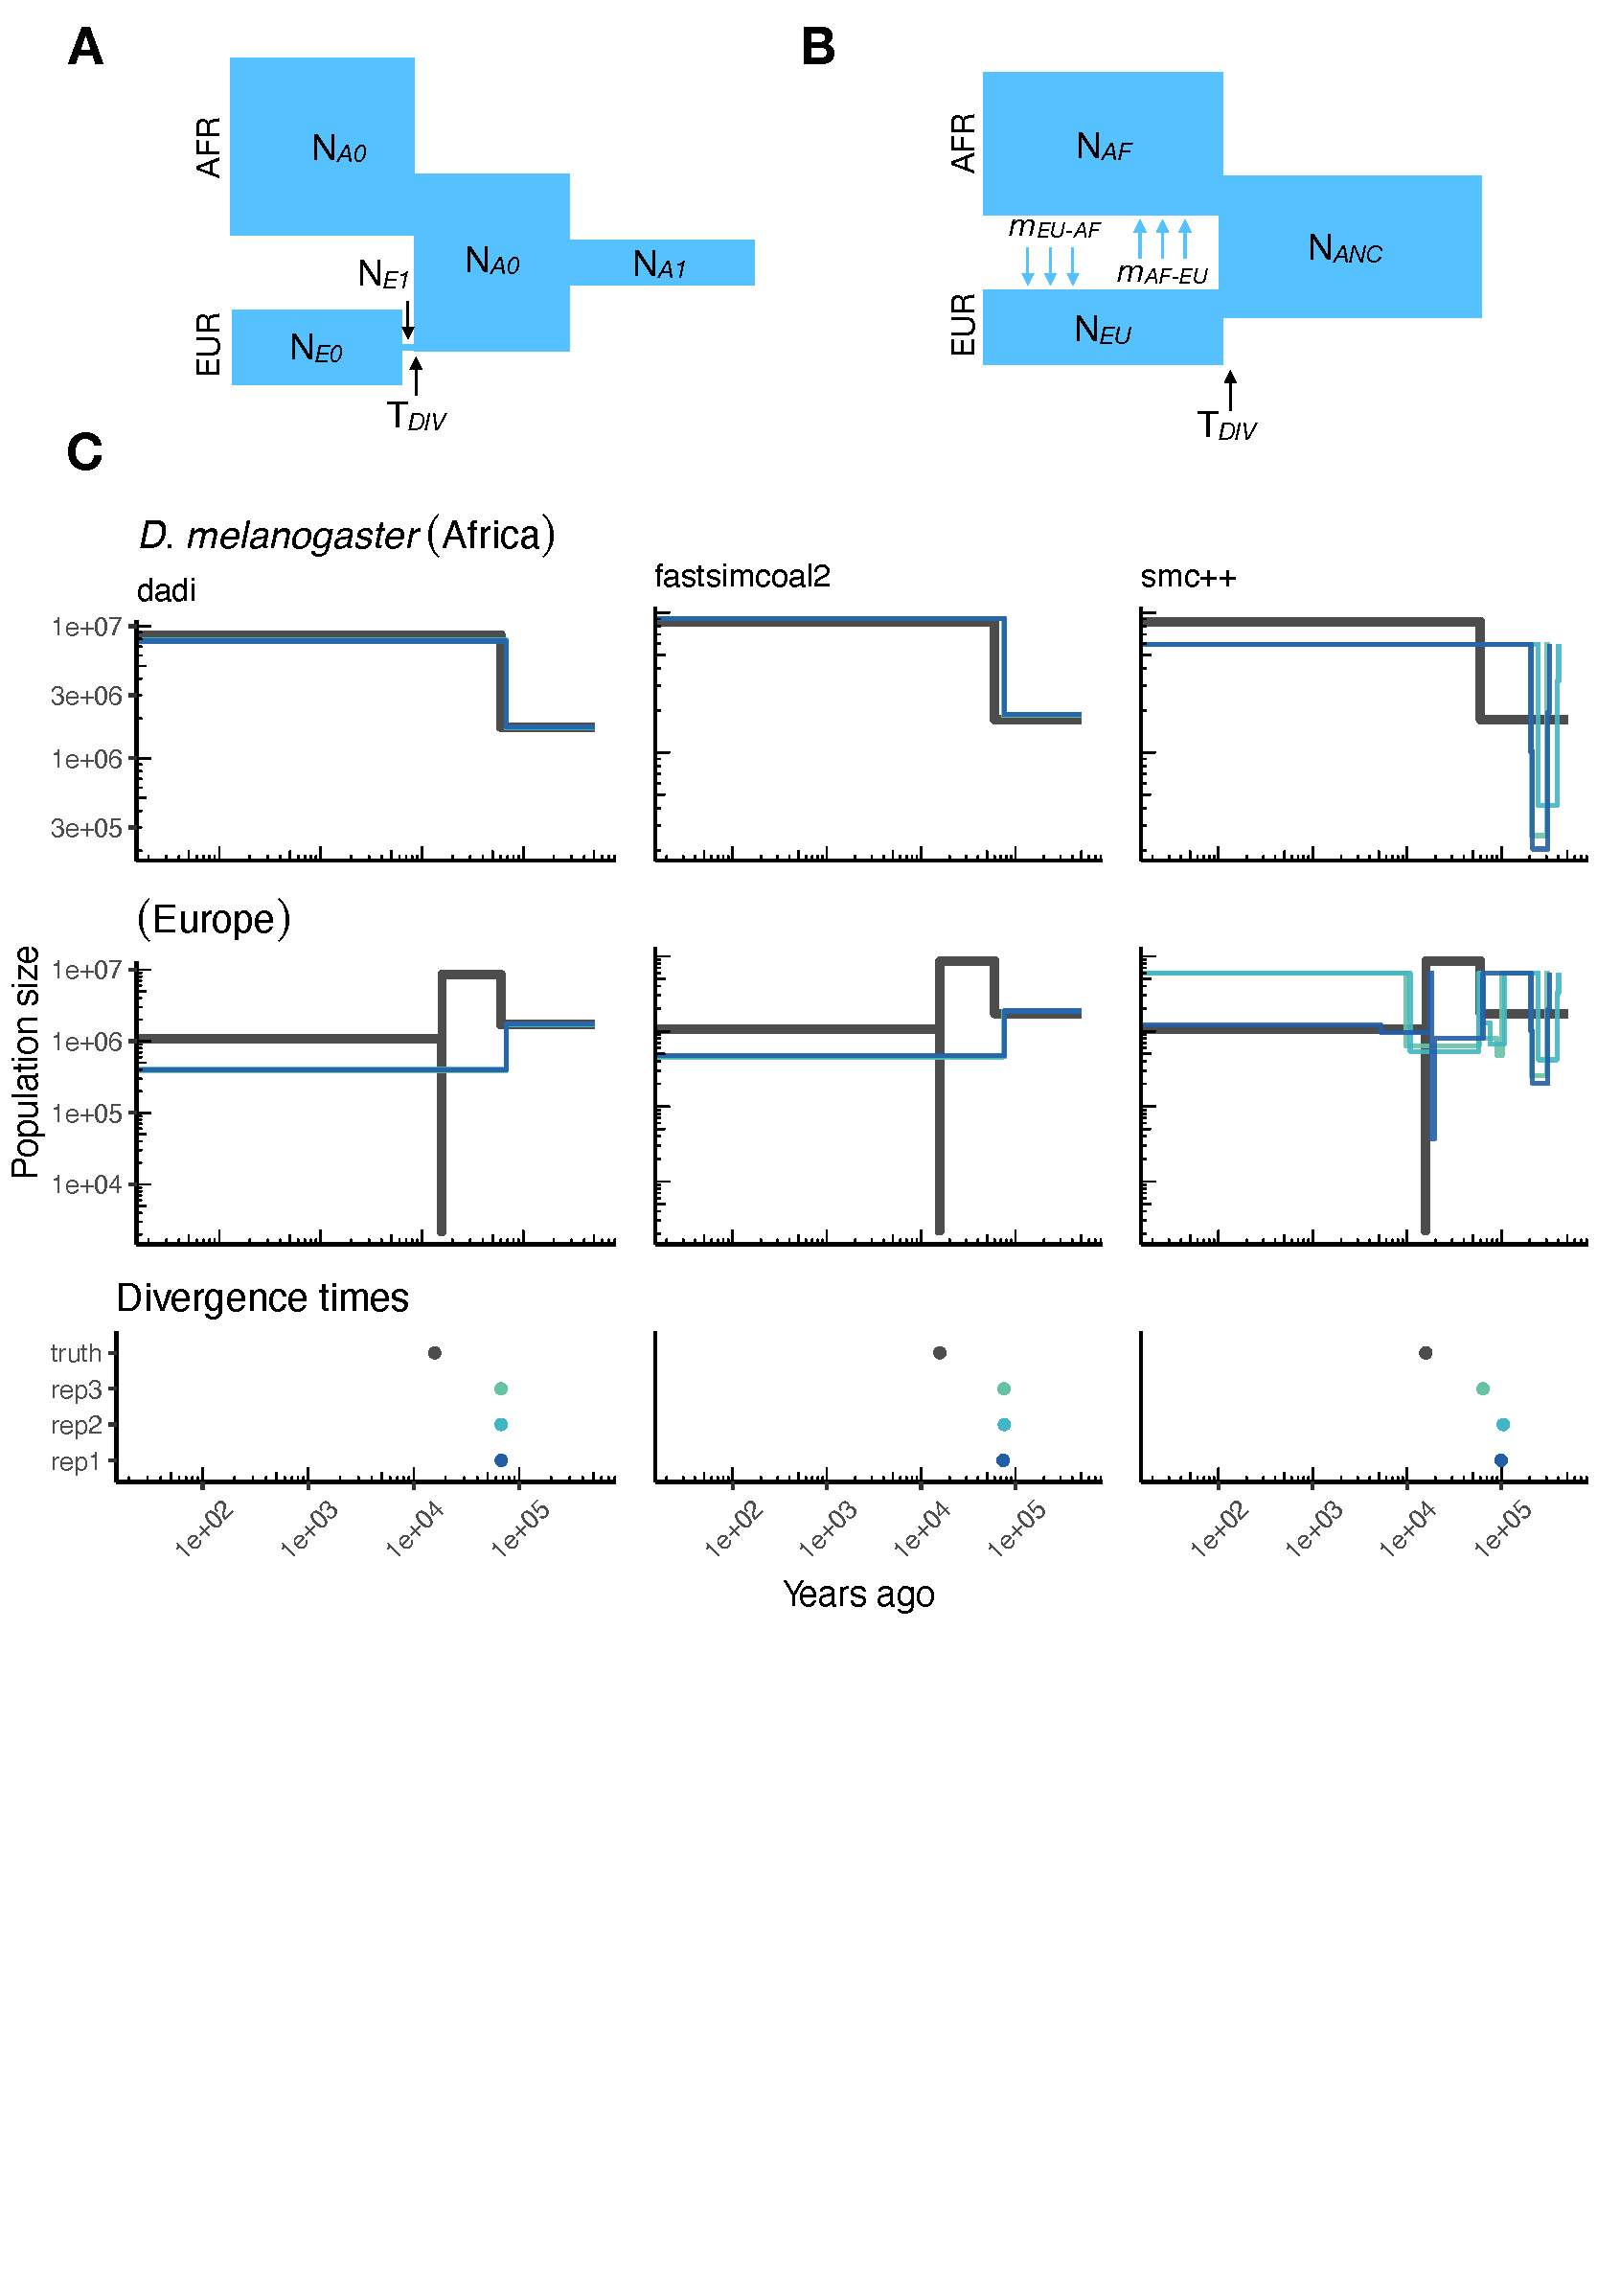
\includegraphics[width=0.8\linewidth]{display_items/d_mel_two_popn_comp.pdf}
\caption{\textbf{Parameters estimated using a two-population \emph{Drosophila} model}.
Here we show estimates of $N(t)$ inferred using \dadi, \fastsimcoal, and \smcpp.
Data were generated by simulating
replicate \emph{Drosophila} genomes under the \cite{li2006inferring} model and using the genetic map
inferred in \cite{comeron2012many}. See legend of Figure \ref{fig:IM_popn_human} for details.
In shades of blue we show the estimated
$N(t)$ trajectories for each replicate. In black we show the simulated population sizes.}
\label{fig:two_popn_fly}
\end{center}
\end{figure}


\begin{figure}
\begin{center}
\includegraphics[width=0.8\linewidth]{display_items/dromel_migration_rates.pdf}
\caption{\textbf{Migration rate parameters estimated under a two-population \emph{Drosophila} model}.
Here we show inferred migration rates from \dadi and \fastsimcoal.
Data were generated by simulating replicate \emph{Drosophila} genomes under the \cite{li2006inferring} model and using the genetic map
inferred in \cite{comeron2012many}.
Directional migration from Europe to Africa is represented as $MIG\_AF\_EU$ and
migration from Africa to Europe is represented as $MIG\_EU\_AF$.
Note that the $x$-axis coordinates are arbitrary.}
\label{fig:dromel_mig_rates}
\end{center}
\end{figure}



\begin{figure}
\begin{center}
\includegraphics[width=0.8\linewidth]{display_items/n_t_dag.pdf}
\caption{\textbf{Workflow for our N(t) inference methods comparison.}
Here we show single replicate for two chromosomes, chr22 and chrX, simulated under the HomSap
OutOfAfrica\_3G09 demographic model, with a HapmapII\_GRCh37 genetic map.
Note that resulting data for input to all inference methods \smcpp, \MSMC, and \stairwayplot,
come from the same set of simulations.}
\label{fig:n_t_dag}
\end{center}
\end{figure}


\begin{figure}
\begin{center}
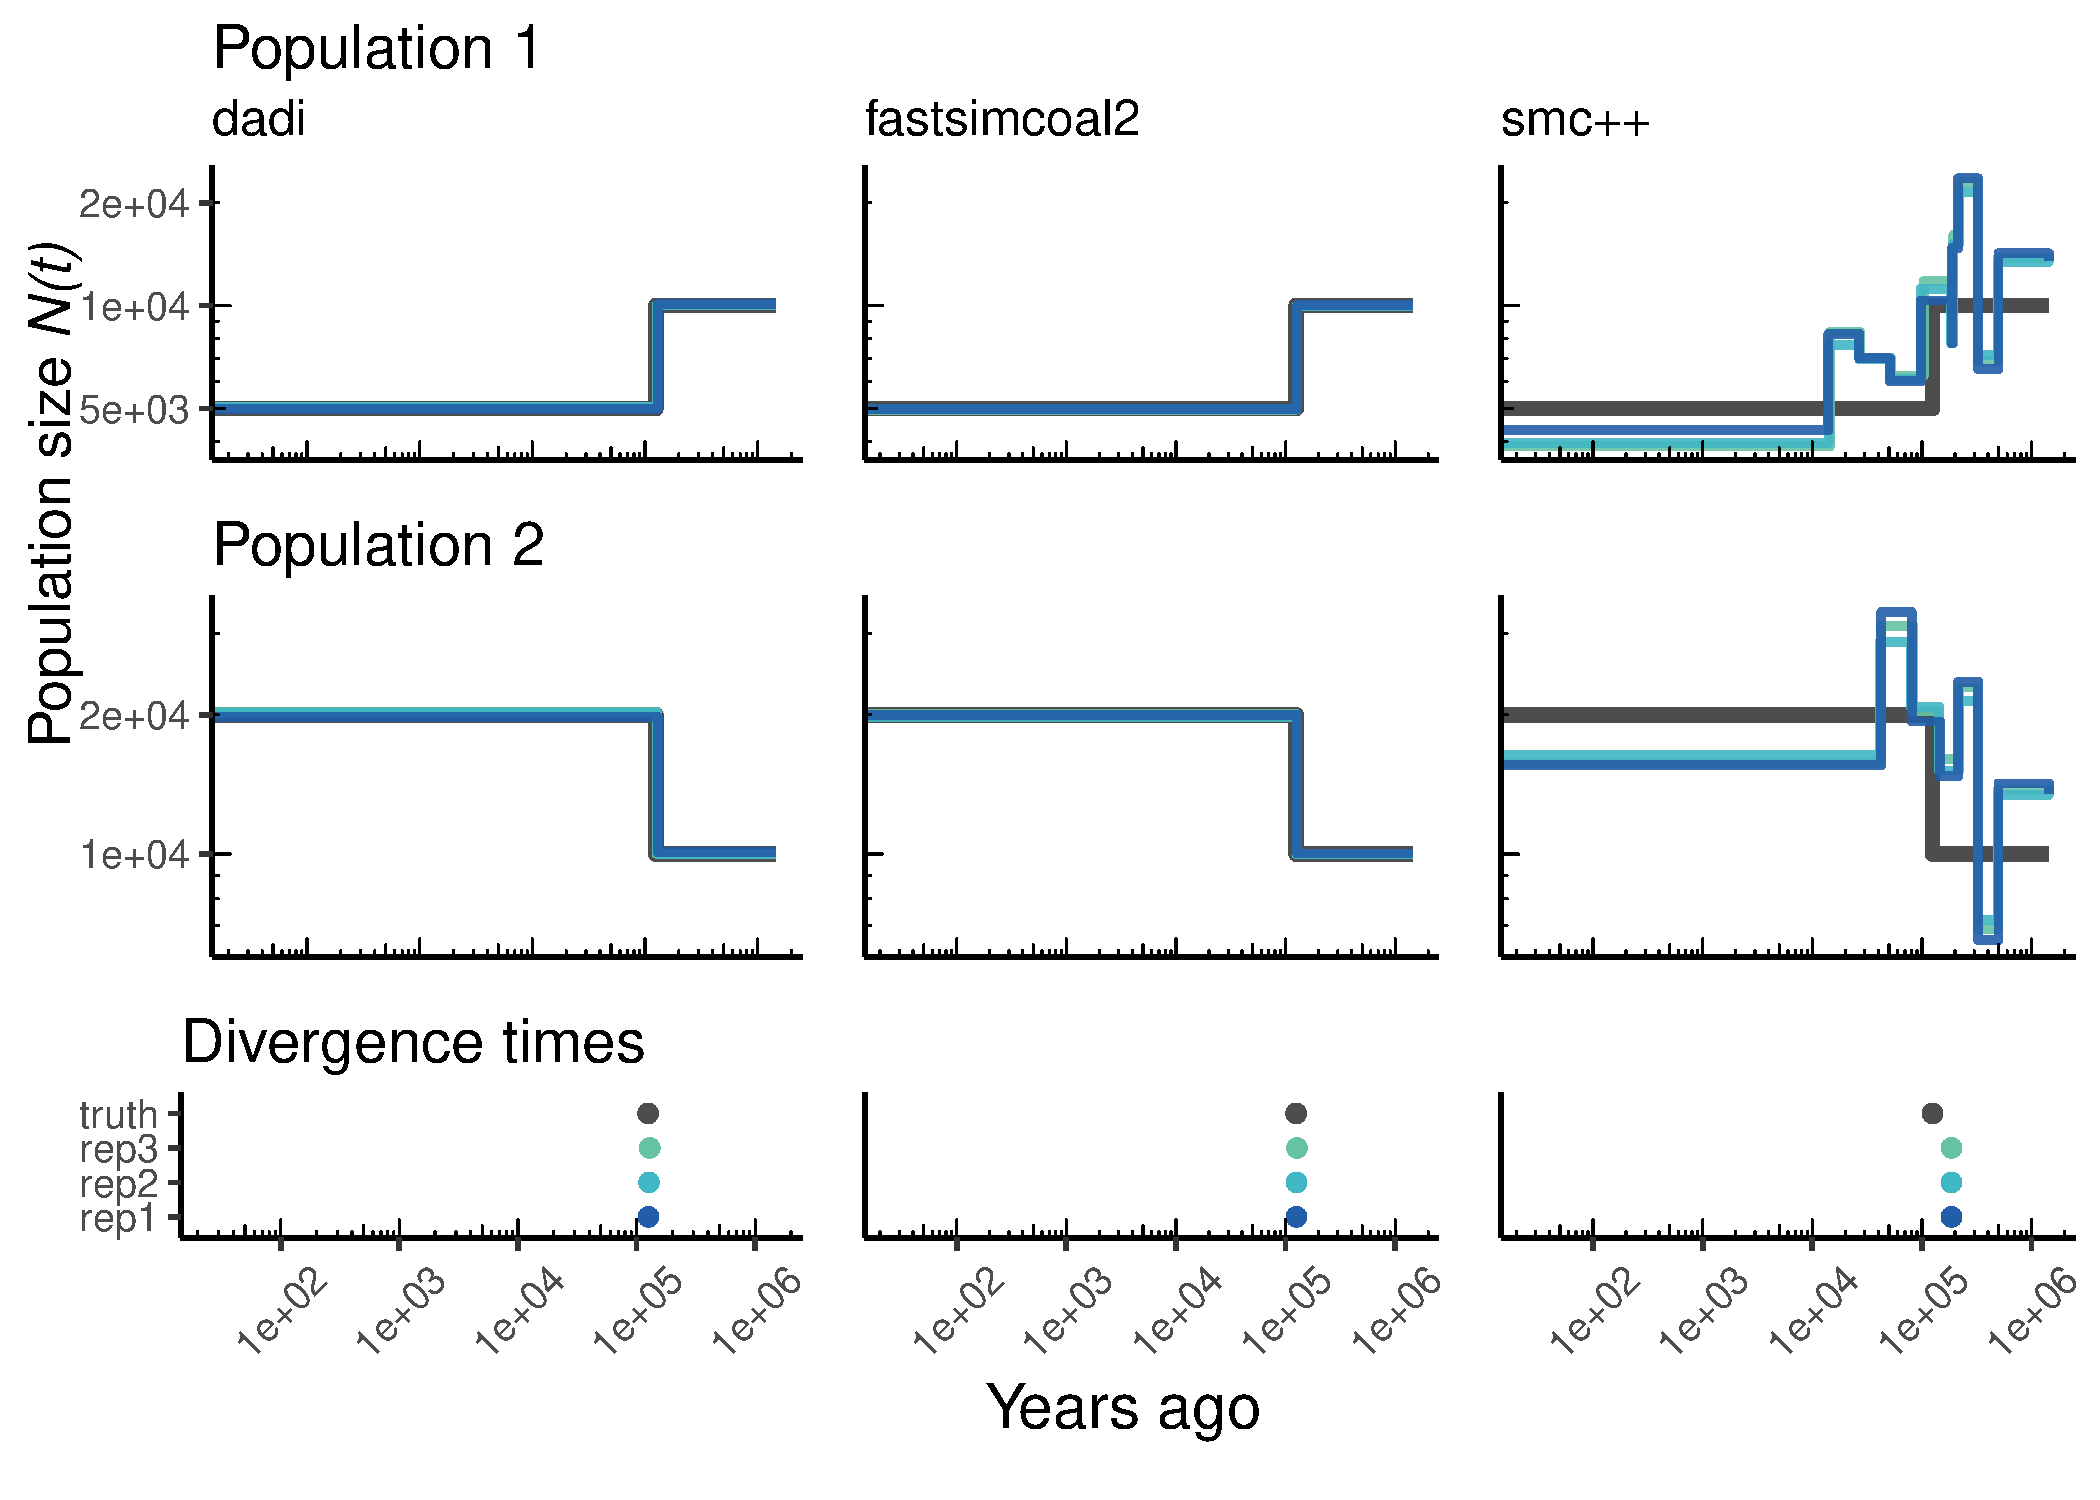
\includegraphics[width=0.8\linewidth]{display_items/generic_IM.pdf}
\caption{\textbf{Parameters estimated from a generic IM model} Here we show estimates of $N(t)$
inferred using \dadi, \texttt{fastsimcoal2}, and \smcpp. Data were generated by simulating
under a generic IM model with a human genome and \cite{international2007second} genetic map.
In shades of blue we show the estimated
$N(t)$ trajectories for each replicate. In black we show the simulated population sizes.}
\label{fig:generic_IM}
\end{center}
\end{figure}



\stopsupplement

\appendix

\section*{Calculating coalescence rates}

We compute the coalescence rate of a collection of samples in a given demographic model
at a particular point back in time
as the expected number of coalescences happening at that time
per unit of time and per pair of as-yet-uncoalesced lineages.
More concretely,
let $p(t)$ denote the probability that the lineages of a randomly chosen pair of samples
have not yet coalesced $t$ units of time ago,
let $p(z, t)$ denote the probability that those lineages have not yet coalesced
and are furthermore both in location $z$,
and let $1/(2 N_e(z,t))$ be the rate of coalescence in location $z$ at the time.
Then, we compute the mean coalescence rate as
$$  r(t)  = \frac{1}{p(t)} \sum_z \frac{p(z,t)}{2N_e(z,t)} . $$
This follows because if we have $n$ diploid samples, and hence $\binom{2n}{2}$ lineages,
the expected number of coalescences in location $z$ between times $t$ and $t+dt$ ago
$$
\binom{2n}{2} p(z,t) \frac{ dt }{ 2 N_e(z,t) },
$$
and the expected number of pairs of uncoalesced lineages at that time is
$$
\binom{2n}{2} p(t) .
$$
The expression for $r(t)$ is a ratio of these two quantities;
to obtain it we need to compute $p(t)$ and $p(z,t)$.
This is relatively straightforward
using the general theory of Markov chains, and is implemented in \texttt{msprime}.

Note that since these quantities are \emph{per pair of lineages},
this definition depends on the locations of the samples.
The coalescence rate also has the intuitive interpretation that
it is the average between-lineage coalescence rate,
averaged over where uncoalesced lineages might be.
Since the local coalescence rate is the inverse of the population size,
$1/r(t)$ (as shown for instance in \autoref{fig:n_t_ragsdale})
is a weighted harmonic mean of the census sizes of the different populations present at that time.
This is as expected: suppose that we have two populations, one big and one small,
connected by migration.
If all our samples are from the big population,
the number of recent coalescences should be small, reflecting the large population size,
while in the long run, the coalescence rate approaches an intermediate rate.
On the other hand, more recent coalescences are expected
if all samples are from the small population,
A method that fits a single, time-varying population size to the data
might be expected to find a population size trajectory
to match these time-varying rates of coalescence.

We use the same computations to analytically compute \emph{mean coalescence times}:
since for any nonnegative random variable $T$, the mean value is
$\mathbb{E}[T] = \int_0^\infty \mathbb{P}\{T > t\} dt$,
we can obtain the mean coalescence time as
$$
\int_0^\infty p(t) dt ,
$$
where $p(t)$ is defined above.

\end{document}
